\section{数值验证、收敛性与灵敏度完整结果}
\begin{figure}[H]\centering
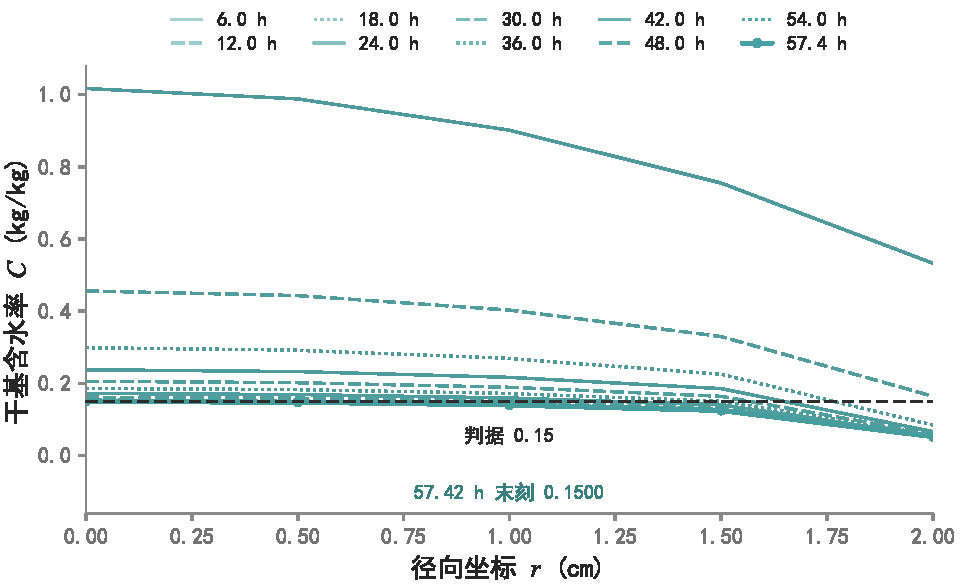
\includegraphics[width=.72\textwidth]{../figures/fig_q3_profiles_6h.pdf}
\caption{问题三每六小时径向剖面}\end{figure}
\subsection{网格和时间步收敛}
\begin{figure}[H]\centering
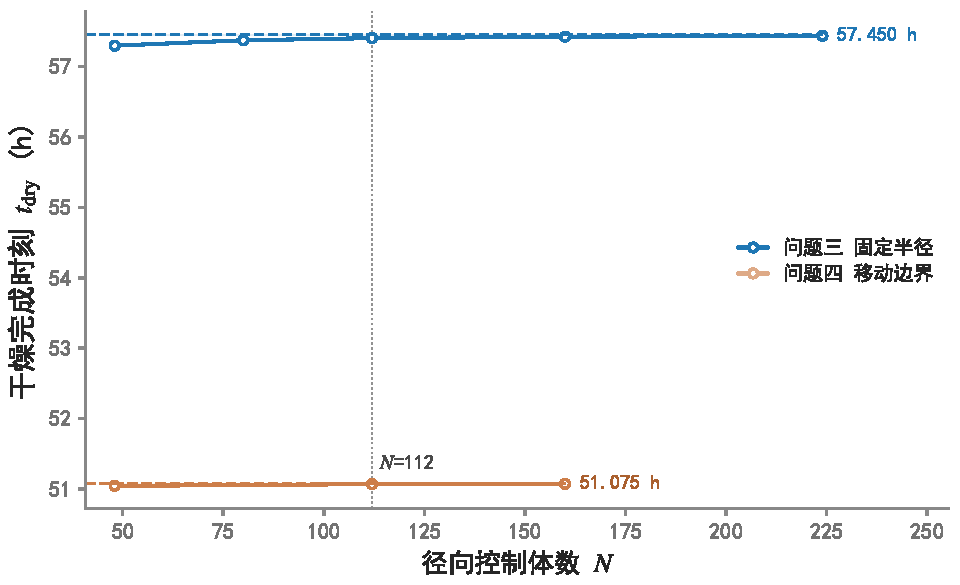
\includegraphics[width=.68\textwidth]{../figures/fig_grid_convergence.pdf}
\caption{问题三、四网格收敛轨迹}\label{fig:grid_convergence}\end{figure}
\begin{table}[H]\centering\small\caption{问题三网格收敛性}\begin{tabular}{rrr}\toprule
$N$&$t_{\mathrm{dry}}$ (h)&相对前一档差(\%)\\\midrule
48&57.2968&--\\80&57.3738&0.1343\\112&57.4040&0.0527\\160&57.4247&0.0360\\224&57.4370&0.0214\\\bottomrule\end{tabular}\end{table}
\begin{table}[H]\centering\small\caption{问题三时间步收敛性}\begin{tabular}{rr}\toprule
$\Delta t$ (s)&$t_{\mathrm{dry}}$ (h)\\\midrule 4.0&57.4067\\2.0&57.4049\\1.0&57.4040\\0.5&57.4036\\\bottomrule\end{tabular}\end{table}

\subsection{结构性退化与守恒检验}
\begin{table}[H]\centering\small\caption{结构性退化检验结果}\begin{tabular}{lcc}\toprule
检验&判据&实测\\\midrule
零输入&$<10^{-10}$&$2.522\times10^{-13}$\\常空气解析&$<10^{-3}$&$2.165\times10^{-4}$\\纯扩散守恒&$<10^{-12}$&$1.132\times10^{-14}$\\收缩关闭&$<10^{-6}$&$0.000\times10^{0}$\\\bottomrule\end{tabular}\end{table}
\begin{table}[H]\centering\small\caption{各问干质量守恒残差}\begin{tabular}{lrr}\toprule
算例&步数&相对残差\\\midrule 问题一&7200&$4.218\times10^{-11}$\\问题二&21600&$2.139\times10^{-11}$\\问题三&206760&$3.425\times10^{-10}$\\问题四&183900&$1.547\times10^{-10}$\\\bottomrule\end{tabular}\end{table}

\subsection{单因子灵敏度完整结果}
\begin{figure}[H]\centering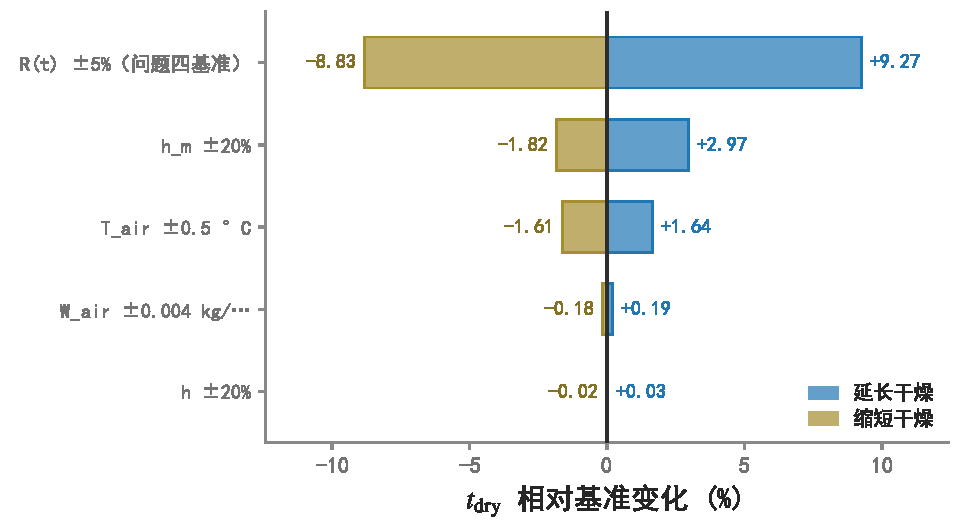
\includegraphics[width=.62\textwidth]{../figures/fig_sensitivity_tornado.pdf}\caption{单因子灵敏度排序}\end{figure}
完整结果表明 $R(t)\gg h_m>T_{\mathrm{air}}\gg W_{\mathrm{air}}\gg h$；半径 $\pm5\%$ 对应时长 $+9.273\%/-8.828\%$，其中心差商弹性为 $1.810$。
